\section{Towards Quantifying the Safety of Soft Robots}
In the following, we contextualize the topic by reviewing the literature on how safety has been assessed and quantified in the realm of robotics before, where almost all prior work is on the safety of industrial and collaborative rigid robotic manipulators.
Subsequently, we will motivate the need for a quantitative safety metric for soft robots by showcasing future applications that such a metric would enable.
This will then allow us to define a list of requirements for characteristics that a safety metric needs to exhibit.

\subsection{Background on Safety Criteria for Robotic Manipulators}

% \textcolor{red}{Stucture: \begin{enumerate}
%     \item Motivation for measuring safety: selecting suitable design, defining constraints that guarantee safety (i.e., ISO norms), and safety-aware control and motion planning
%     \item Stress that this is a well-established line of research in (rigid) robotics involving both conceptual and experimental analysis
%     \item Modes of impact and injury: constrained vs. unconstrained (human), static vs. dynamic, sharp surfaces, different body parts, etc.~\citep{haddadin2009requirements}
%     \item Injurity severity criterias: the first were based on automobile crash models (HIC), but found to be unsuitable as they are calibrated for higher velocities and inertias that are not even relevant for rigid robots. In particular, taking the head acceleration as a injury criteria is not suitable, as not in practice reached, even when robots are moving at 2m/s. Furthermore, it mostly focuses on the question of fatale impacts. Instead, other injury modes, even if not fatal, become relevant as (rigid) robots can still cause bones to break and other significant injuries at their speeds. There exist specialized injury severity criteria inspired by biomechanics for the various body parts. For example, body parts have different contact stiffnesses and injury is (most likely) caused when different thresholds are exceeded (e.g., penetration depth, maximum force, energy density, acceleration). However, it seems that most of them are correlated with the the maximum force experienced during impact and that the maximum force generalizes the best across body parts.
%     \item Mention ISO/TS 15066:2016 (Collaborative robots) and ISO/PAS 5672:2023
%     \item Safety metrics for soft robots: basically not existing, only~\citep{abidi2017intrinsic}, but only super-simplified beam model. A safety metric is especially important for soft robots as we continuously stress the inherent safety of soft robots, so we also need to be able to quantify it.
% \end{enumerate}}

% A safety criterion is defined as quantifying the (potential) injury severity that is caused during the collision between a machine and a human~\citep{haddadin2013towards}.
% As the existing literature on quantifying the safety of soft robots is extremely limited~\citep{abidi2017intrinsic}, we will in the following mostly focus on the related work on deriving safety criterias for rigid, and specifically collaborative, robots~\citep{zinn2004playing, de2008atlas, haddadin2013towards}.
% Specifically, we want to highlight here the seminal work by \citet{haddadin2013towards} and the established international regulations for ensuring safe robot (e.g., \gls{Cobot}) behavior in collaborative settings between humans and robots.
A safety criterion is defined as a measure of the potential injury severity resulting from a collision between a machine and a human~\citep{haddadin2013towards}. Given the scarcity of literature on the safety quantification of soft robots~\citep{abidi2017intrinsic}, we will primarily concentrate on work related to establishing safety criteria for rigid, and specifically collaborative, robots~\citep{zinn2004playing, de2008atlas, haddadin2013towards}. In particular, we want to highlight the seminal work by \citet{haddadin2013towards} as well as the established international regulations that ensure safe robot (e.g., \gls{Cobot}) behavior in collaborative human-robot settings.

\subsubsection{Motivation}

% Various aspects have motivated the robotic community to try to assess the safety of our robots and develop such safety criteria~\citep{de2008atlas, van2018spatial}: 
% First of all, understanding the important factors influencing safety allows us to make robotic designs and control algorithms safer~\citep{bicchi2004fast, zinn2004new, albu2007dlr, bischoff2010kuka, park2011designing, mansfeld2018safety}. 
% Secondly, quantifying the injury risk stemming from a robot allows the establishment of minimal safety standards and specifically constraints on the design and actuation that guarantee safe deployment of the robots, as done, for example, in ISO 10218-1:2011~\citep{iso2011industrial} for industrial robots and ISO/TS 15066:2016~\citep{iso2016collaborative} for collaborative robots. This allows the designers and manufacturers of robots to certify that their design is \emph{safe}, which is, in turn, crucial for successful adoption by industrial customers and consumers.
% Thirdly, modeling the injury risk of robots and explicitly setting operation constraints that guarantee safety enables safety-aware control and motion planning~\citep{lacevic2011safety, haddadin2013towards, iso2016collaborative, bertino2023prescribed, ferraguti2020control, lacevic2022safe, pupa2024efficient}.
% There exist various approaches to achieving such safety-aware control.
% Very established and already proposed early on were collision avoidance algorithms~\citep{haddadin2013towards} that cause the robot to perform an evasive motion when contact/collision is noted by a force/torque observer~\citep{de2006collision, haddadin2008collision, haddadin2011study}. However, this collision avoidance approach exhibits various disadvantages, such as, by definition a reactive behavior where, in some situations, injuries cannot be avoided as a consequence of time delays (e.g., observer and reaction time deal) and actuator limits (i.e., the inertia of the system doesn't allow the robot to be stopped quickly enough). Furthermore, avoiding contact in general is in conflict with the vision of humans and robots collaborating closely together.
% To counter these shortcomings, the alternative is to consider the safety criteria directly for control and motion planning~\citep{haddadin2013towards}.
% One common approach is to define kinematic constraints such that safety is always ensured. Such kinematic constraints can operate either on the joint-space/task-space positions of the robot, also referred to in the literature as danger zones~\citep{lacevic2011safety, lacevic2022safe}, ensuring a safe separation distance from the human~\citep{iso2016collaborative}, which ensure that robot can always be slowed/stopped in time to ensure safety. Then, either the robot is not able to in areas of the workspace that are designated as unsafe, which can be, for example, accomplished using safety filters~\citep{haddadin2010real, bertino2023prescribed}, or alternatively, the human needs to keep out of such unsafe zones when the robot is operating there. Alternatively, such kinematic constraints can also be directly defined as maximum joint- or task-space velocities~\citep{ferraguti2020control, pupa2024efficient, iso2016collaborative}, which can be ensured via direct saturation or optimization-based techniques, such as \gls{MPC})~\citep{pupa2024efficient}, or \gls{CBF}~\citep{ferraguti2020control}, that aim to preserve the desired task behavior~\citep{haddadin2010real}. Finally, also dynamic constraints (e.g., maximum contact force/pressure) could be formulated and ensured via \gls{MPC}, \glspl{CBF}~\citep{ames2016control}, or more safety filters~\citep{hewing2020learning}.

Various factors have motivated the robotics community to assess robot safety and develop corresponding criteria~\citep{de2008atlas, van2018spatial}. 
First, by understanding the key safety-related factors, we can enhance robotic designs and control algorithms~\citep{bicchi2004fast, zinn2004new, albu2007dlr, bischoff2010kuka, park2011designing, mansfeld2018safety}. Second, quantifying the injury risks associated with robots enables the establishment of minimal safety standards and constraints on design and actuation—illustrated, for instance, by ISO 10218-1:2011~\citep{iso2011industrial} for industrial robots and ISO/TS 15066:2016~\citep{iso2016collaborative} for collaborative robots. This process allows designers and manufacturers to certify that their designs are \emph{safe}, which is crucial for adoption by industrial customers and consumers. Third, modeling injury risk and explicitly setting operational constraints paves the way for safety-aware control and motion planning~\citep{lacevic2011safety, haddadin2013towards, iso2016collaborative, bertino2023prescribed, ferraguti2020control, lacevic2022safe, pupa2024efficient}.

There are several approaches to achieving such safety-aware control. One well-established method is the use of collision avoidance algorithms~\citep{haddadin2013towards}, which trigger evasive maneuvers when a force/torque observer detects contact or collision~\citep{de2006collision, haddadin2008collision, haddadin2011study}. However, this reactive approach has its drawbacks—time delays (from observation and reaction times) and actuator limitations (due to system inertia) may sometimes prevent injuries from being avoided. Moreover, aiming to avoid contact altogether runs counter to the vision of close human-robot collaboration.

To address these shortcomings, another strategy is to incorporate safety criteria directly into control and motion planning~\citep{haddadin2013towards}. A common approach is to define kinematic constraints that inherently ensure safety. These constraints can be applied to the robot’s joint-space or task-space positions—often referred to as danger zones in the literature~\citep{lacevic2011safety, lacevic2022safe}—to maintain a safe separation distance from humans~\citep{iso2016collaborative} and ensure that the robot can always be slowed or stopped in time. This can be achieved either by preventing the robot from entering unsafe areas, for example, using safety filters~\citep{haddadin2010real, bertino2023prescribed}, or by requiring humans to steer clear of these zones during operation. Alternatively, kinematic constraints can be defined in terms of maximum joint- or task-space velocities~\citep{ferraguti2020control, pupa2024efficient, iso2016collaborative}, enforced via direct saturation or optimization-based techniques—such as \gls{MPC}~\citep{pupa2024efficient} or \gls{CBF}~\citep{ferraguti2020control}—which aim to preserve the desired task behavior~\citep{haddadin2010real}. Finally, dynamic constraints (e.g., maximum contact force or pressure) may also be formulated and enforced through \gls{MPC}, \glspl{CBF}~\citep{ames2016control}, or additional safety filters~\citep{hewing2020learning}.

\subsubsection{Classification of Collisions}

% Collisions between robots and humans can most generally be classified into \emph{blunt} and \emph{sharp} contact~\citep{haddadin2009requirements, haddadin2011safe, haddadin2013towards}. In blunt contact, the robot makes contact with a human using a large, flat, or rounded surface. The force is distributed over a wider area, which may reduce the likelihood of penetration but can still result in injuries such as bruises, contusions, lacerations (crush and gash), internal injuries or even fractures if the impact energy is high~\citep{haddadin2009requirements, haddadin2011safe, haddadin2013towards}. In the case of sharp and acute contact, the robot touches the human with a small, focused area—such as a point, edge, or any protruding element with a fine geometry. Because the force is concentrated on a smaller area, sharp contact has a higher potential for causing lacerations (cut and stab/puncture) or abrasions wounds. These types of contacts are particularly hazardous because even a relatively low force can result in severe injuries~\citep{haddadin2010soft, haddadin2011study}.
% However, as sharp contact is most often caused by the the tool use and otherwise sharp contact along the body of the (soft) robot it can be relatively easily avoided by appropriate material choices\footnote{Actually, in many cases, according to \citet{haddadin2011study}, similiar (force-based) techniques can be to derive safety criteria for sharp than for blunt contacts. The main difference is, that the relevant thresholds for safe behavior need to be adjusted. For example, pain/injury tolerance for uncovered skin lies at $75 \pm 45 \si{N}$ and $12.4 \pm 4.9 \si{mm}$ with respect to forces and deflection, respectively~\citep{haddadin2010soft, haddadin2011study}.}, we will in the following mostly focus instead on reviewing the literature on safety criteria for \emph{blunt} contacts~\citep{haddadin2011study, haddadin2013towards}.
% Generally, the injury severity needs to be analyzed separately for each body part  (e.g., head, neck, chest, arm, eye, etc.)~\citep{haddadin2008collision, haddadin2013towards} separately and it is common for safety criteria to exist that a specialized on representing the injury severity of the impact on a specific body part\footnote{One exception for this are soft-tissue injuries caused by sharp contact which typically generalize across various body parts (with the exception of the eye), with only the lethal penetration depth varying~\citep{haddadin2010soft, haddadin20111
% }.}~\citep{haddadin2009requirements, haddadin2011safe, haddadin2013towards}.
% Finally, collisions can be further classified according to to the contact scenario, including quasi-static vs. dynamic, and if injuries occur as a result of direct impact, clamping in the robot structure, or the human is harmed because of a secondary impact with the environment as a consequence of the collision with the robot~\citep{haddadin2009requirements, haddadin2011safe}.
Collisions between robots and humans are generally categorized as either blunt or sharp contacts~\citep{haddadin2009requirements, haddadin2011safe, haddadin2013towards}. In blunt contact, the robot engages with a human using a large, flat, or rounded surface, which spreads the force over a broader area. Although this distribution may lower the risk of penetration, it can still lead to injuries—such as bruises, contusions, lacerations (both crush and gash), internal injuries, or even fractures—if the impact energy is sufficiently high~\citep{haddadin2009requirements, haddadin2011safe, haddadin2013towards}. Conversely, sharp or acute contacts occur when the robot makes contact with a small, focused area, like a point, edge, or any protruding element with a fine geometry. Because the force is concentrated over a smaller area, sharp contact has a greater potential for causing lacerations (cuts, stabs, or punctures) or abrasion wounds, making even relatively low forces particularly dangerous~\citep{haddadin2010soft, haddadin2011study}.

Since sharp contact is most often caused by tool use or by other sharp elements along the body of a (soft) robot, it can typically be avoided through an appropriate robot surface design\footnote{According to \citet{haddadin2011study}, similar force-based techniques can be used to derive safety criteria for sharp contacts as for blunt contacts, with the primary difference being that the relevant safety thresholds need to be adjusted. For example, the pain/injury tolerance for uncovered skin is approximately $75 \pm 45 \si{N}$ and $12.4 \pm 4.9 \si{mm}$ for forces and deflection, respectively~\citep{haddadin2010soft, haddadin2011study}.}. Consequently, our focus will primarily be on reviewing literature related to safety criteria for blunt contacts~\citep{haddadin2011study, haddadin2013towards}. Typically, injury severity is analyzed separately for each body part (e.g., head, neck, chest, arm, eye, etc.)~\citep{haddadin2008collision, haddadin2013towards}, and safety criteria are often specialized to represent the injury severity on a specific area\footnote{One exception is soft-tissue injuries caused by sharp contact, which generally apply across various body parts (except for the eye), with the main variation being the lethal penetration depth~\citep{haddadin2010soft, haddadin2011study}.}. Finally, collisions can also be classified based on the contact scenario, distinguishing between quasi-static and dynamic interactions, and considering whether injuries result from direct impact, clamping within the robot structure, or secondary impacts with the environment following the collision~\citep{haddadin2009requirements, haddadin2011safe}.
%
% The safety criteria, also commonly referred to injury severity criteria, that have been so far proposed for rigid robots can be generally classified into acceleration-, force-, stress/pressure, compression-, viscous-, and energy-based criteria~\citep{haddadin2009requirements, haddadin2013towards}.

\subsubsection{Safety Criteria for Collaborative Robots}

The safety criteria—often referred to as injury severity criteria—that have been proposed for rigid robots can be broadly categorized into acceleration-, force-, stress/pressure-, compression-, viscous-, and energy-based criteria~\citep{haddadin2009requirements, haddadin2013towards}.

% \textbf{Acceleration-based criteria} are in particular commonly adapted for assessing the severity of head injuries, but also find adoption for chest injuries~\citep{haddadin2013towards}.
% The the vast number of proposed acceleration-based head injury severity criteria were originally proposed for automotive applications. Prominent examples are the \SI{3}{ms}-Criterion which ask for the maximum \SI{3}{ms}-average of the head acceleration over the collision duration to be less than \SI{72}{g}~\citep{got1978results, haddadin2013towards}. Another very prominent example, and the most frequently adopted head severity index, is the \gls{HIC}~\citep{versace1971review} which considers an the maximum of the acceleration integrated over a duration of \SI{36}{ms} encountered during the collision~\citep{haddadin2013towards}. To the best of our knowledge, the first adaption of the \gls{HIC} within the robotics community~\citep{bicchi2004fast, zinn2004playing, zinn2004new}, later also investigated by \citet{haddadin2008role, bicchi2008physical, shin2008hybrid}, actually kickstarted the research movement of the development safety criteria for rigid robotic manipulators\citep{de2008atlas, haddadin2013towards}.
% However, later research found that many injury severity criteria developed originally with automative applications in mind, and in particular the \gls{HIC}, cannot be very meaningfully used as a safety criterion for collaborative robots as (a) they are poorly calibrated for the acceleration encountered during human-robot collisions, (b) even when the \glspl{Cobot}~\citep{albu2007dlr, bischoff2010kuka} move at their maximum speed, the injury level doesn't register on the EuroNCAP~\citep{EuroNCAP2004} scale leading to an assessment of \emph{very low} injury-level, which might be a good outcome for (hopefully) rather rare car crashes, but can still translate to pain or even minor injuries, which is not acceptable when we want humans to collaborate with robots~\citep{haddadin2009requirements, haddadin2011safe}.
\textbf{Acceleration-based criteria} are commonly employed to assess head injuries and, to a lesser extent, chest injuries~\citep{haddadin2013towards}. Most acceleration-based head injury severity measures were originally developed for automotive applications. For instance, the \SI{3}{ms} Criterion requires that the maximum \SI{3}{ms}-average head acceleration during a collision remains below \SI{72}{g}~\citep{got1978results, haddadin2013towards}. Another notable example—and the most widely adopted head injury index—is the \gls{HIC}~\citep{versace1971review}, which evaluates the maximum acceleration integrated over a \SI{36}{ms} period during a collision~\citep{haddadin2013towards}. To our knowledge, the first adaptation of the \gls{HIC} for the robotics community~\citep{bicchi2004fast, zinn2004playing, zinn2004new}, later explored further by \citet{haddadin2008role, bicchi2008physical, shin2008hybrid}, spearheaded the research on safety criteria for rigid robotic manipulators~\citep{de2008atlas, haddadin2013towards}. However, subsequent studies have shown that many injury severity criteria originally designed for automotive use—and in particular the \gls{HIC}—are not well-suited as safety measures for collaborative robots because (a) they are not properly calibrated for the accelerations typical in human–robot collisions but instead are focused assessing the fatality of impacts, and (b) even when the robots operate at maximum speed, which is approximately \SI{2}{m \per s}~\citep{haddadin2009requirements} for common \glspl{Cobot}~\citep{albu2007dlr, bischoff2010kuka}, the resulting injury level is assessed as very low on the EuroNCAP~\citep{EuroNCAP2004} scale. While this might be acceptable for the relatively rare car crashes, even minor injuries are unacceptable in human–robot collaboration settings~\citep{haddadin2009requirements, haddadin2011safe}.

% \textbf{Force-based criteria} consider the (maximum) contact force experienced during the collision and are frequently applied for assessing the severity of neck and chest injuries~\citep{haddadin2013towards}. For the neck, the automative literature, EuroNCAP~\citep{EuroNCAP2004}, cites a critical value of \SI{1100}{N} based on biomechanical and forensic tests~\citep{madea2019handbuch, haddadin2009requirements}.
% ISO/TS 15066:2016~\citep{iso2016collaborative} sets the threshold for minor injuries based on biomechanical studies with adults~\citep{muttray2014kollaborierende} at $65-300~\si{N}$ quasi-static contact force, where the lowest pain threshold applies to the face.
% It is important to note that in transient scenarios, the humans are willing to accept roughly 2x as high forces.
% In these tests, a contact area of $\sim 2~\si{N \per cm^2}$ was considered~\citep{iso2016collaborative}.
\textbf{Force-based criteria}~\citep{kirschner2021experimental} evaluate the (maximum) contact force experienced during a collision and are often used to assess the severity of neck and chest injuries~\citep{haddadin2013towards}. In automotive literature, EuroNCAP~\citep{EuroNCAP2004} cites a critical neck force of \SI{1100}{N} based on biomechanical and forensic studies~\citep{madea2019handbuch, haddadin2009requirements}. ISO/TS 15066:2016~\citep{iso2016collaborative} establishes a threshold for minor injuries—derived from biomechanical studies with adults~\citep{muttray2014kollaborierende}—at quasi-static contact forces of $65-300~\si{N}$, with the lowest pain threshold applying to the face. It is important to note that in transient scenarios, humans can tolerate roughly twice these force levels. In these assessments, a contact area of approximately $\sim 2~\si{cm^2}$ is assumed~\citep{iso2016collaborative}.

% \textbf{Pressure/stress-based criteria} are closely relate as they consider the maximum (local) ratio between contact force and contact area. According to the ISO norm~\citep{iso2016collaborative}, they are relevant for the assessment of the pain sensitivity and injury severity of blunt impacts on the vast majority body parts, with the threshold according to biomechanical pain tolerance studies~\citep{muttray2014kollaborierende} set at $1.1-3~\si{MPa}$ for quasi-static contact. 
% Here, the peak pressure was measured with a resolution of \SI{1}{mm^2}~\citep{iso2016collaborative}.
\textbf{Pressure/stress-based criteria}~\citep{wassink2007towards, haddadin2013towards} are closely related to force-based criteria, as they assess the maximum local ratio of contact force to contact area. According to the ISO norm~\citep{iso2016collaborative}, these criteria are pertinent for evaluating pain sensitivity and injury severity from blunt and even sharp impacts across most body parts. Biomechanical pain tolerance studies~\citep{muttray2014kollaborierende} have set the quasi-static contact threshold at $1.1-3~\si{MPa}$, with peak pressures measured at a resolution of \SI{1}{mm^2}~\citep{iso2016collaborative}.

% \textbf{Compression-based criteria} are particular prevalently used for modeling chest injuries~\citep{haddadin2013towards}. For example, the Compression Criterion~\citep{lobdell1973impact, kroell1974impact} requires the maximum deformation of the chest to remain below \SI{22}{mm}.
% \textbf{Viscous-based criteria} consider in addition to the (chest) deformation also the corresponding velocity. For example, the Viscous Criterion~\citep{viano1985thoracic, lau1986viscous}, also known as soft-tissue criterion, takes the product between the two, but is suspectible to measurement noise~\citep{haddadin2011safe}.
% \textbf{Energy-based criteria} consider the (kinetic) energy transferred to the human as a result of the collision with the robot~\cite{haddadin2011safe, haddadin2013towards, iso2016collaborative}. 
% While such energy criteria has in particular been used to assess the injury severity of head impacts~\citep{haddadin2009requirements}, with already a transferred kinetic energy of $50-100~\si{J}$ leading to a fracture of the scull~\citep{haddadin2009requirements}, limits on the maximum transferred energy have also been established in ISO/TS 15066:2016~\citep{iso2016collaborative} for other body parts - usually lying around $\SI{0.1}{J}$ (face) and $\SI{2.6}{J}$ (pelvis).
% While the benefit of this safety criterion is to consider not just, for example, the (peak) contact pressure at a point in time, but instead integrating this over a transient which has been shown to be relevant~\citep{iso2016collaborative}, a disadvantage is that it cannot incorporate knowledge about contact area (e.g., blunt vs. sharp contacts), which clearly has in practice an impact on the injury severity.
% This is resolved when instead considering normalized energy, also referred to as energy density, where the threshold lies at $\SI{2.5}{J \per cm^2}$ for soft tissue~\citep{haddadin2011safe}. Also, energy density has been shown to be a good indicator for eye injuries~\citep{haddadin2013towards}.
\textbf{Compression-based criteria} are particularly prevalent for modeling chest injuries~\citep{haddadin2007safety, haddadin2013towards}. For instance, the Compression Criterion~\citep{lobdell1973impact, kroell1974impact} stipulates that the maximum chest deformation should not exceed \SI{22}{mm}.
%
\textbf{Viscous-based criteria} take into account not only the (chest) deformation but also the associated velocity~\citep{haddadin2007safety, haddadin2013towards}. An example is the Viscous Criterion~\citep{viano1985thoracic, lau1986viscous}, also known as the soft-tissue criterion, which multiplies these two factors; however, it is prone to measurement noise~\citep{haddadin2011safe}.

\textbf{Energy-based criteria} evaluate the (kinetic) energy transferred to a human during a collision with the robot~\citep{haddadin2011safe, haddadin2013towards, iso2016collaborative}. Such energy criteria have been used particularly to assess head injury severity~\citep{haddadin2009requirements}, where a kinetic energy transfer of just $50-100~\si{J}$ can fracture the skull~\citep{haddadin2009requirements}. Additionally, ISO/TS 15066:2016~\citep{iso2016collaborative} has set maximum transferred energy thresholds for other body parts—approximately $\SI{0.1}{J}$ for the face and $\SI{2.6}{J}$ for the pelvis. Although the strength of this safety criterion lies in its integration of transient forces over time, rather than just considering the (peak) contact pressure at a single moment, a drawback is that it does not factor in the contact area (e.g., blunt versus sharp contacts), which significantly influences injury severity in practice. This limitation is addressed by considering normalized energy, also known as energy density, where the threshold is set at $\SI{2.5}{J \per cm^2}$ for soft tissue~\citep{haddadin2011safe}. Energy density has also proven to be an effective indicator for eye injuries~\citep{haddadin2013towards}.

% The collision between the robot and a human (body part) is usually modelled by considering two point masses $m_\mathrm{R}$ and $m_\mathrm{H}$, respectively, that are separated by a spring which accounts for the serial elasticity of the robot surface and the human soft tissue~\citep{haddadin2009requirements, iso2016collaborative}.
% This approach allows straightforward evaluation of all previously introduced safety criteria, as, for example, the contact force is given by the evolution of the spring force in time.
% The point mass of the robot $m_\mathrm{R}$ is given by evaluating the reflected inertia of the system at a given position by formulating the operation-space dynamics~\citep{khatib1987unified} (see Section~\ref{sub:background:dynamics:task_space} for more details).
% The reflected inertia of the human $m_\mathrm{H}$ is stated for various body parts in ISO/TS 15066:2016~\citep{iso2016collaborative}. However, this is only relevant when considering contact scenarios where the human is unconstrained in its motion (i.e., is free to recoil)~\citep{haddadin2009requirements}. Instead, collision scenarios where the human is (partially) constrained typically lead to much larger injury severities. To capture the \emph{worst-case} of the human body part being fully constrained~\citep{haddadin2009requirements, haddadin2011safe}, we can assume $m_\mathrm{H} \gg m_\mathrm{R}$.
The collision between a robot and a human (or a specific body part) is typically modeled by representing them as two point masses, $m_\mathrm{R}$ and $m_\mathrm{H}$, connected by a spring that captures the serial elasticity of both the robot’s surface and the human soft tissue~\citep{bicchi2004fast, haddadin2009requirements, iso2016collaborative}. This model facilitates the straightforward evaluation of the safety criteria introduced earlier, since, for example, the contact force is determined by the evolution of the spring force over time. The robot’s effective mass, $m_\mathrm{R}$~\citep{kirschner2021notion}, is obtained by evaluating the system’s reflected inertia at a given position using operational-space dynamics~\citep{khatib1987unified} (see Section~\ref{sub:background:dynamics:operational_space} for further details). The reflected inertia of the human, $m_\mathrm{H}$, is provided for various body parts in ISO/TS 15066:2016~\citep{iso2016collaborative}. However, this value is relevant only for contact scenarios in which the human is free to move (i.e., unconstrained). In contrast, collision scenarios involving a (partially) constrained human typically result in significantly higher injury severities. To represent the worst-case scenario—where the human body part is completely constrained~\citep{haddadin2009requirements, haddadin2011safe}—we would assume that $m_\mathrm{H} \gg m_\mathrm{R}$.

% Finally, we restate that safety criteria for rigid manipulators operating in human environments (e.g., \glspl{Cobot}) have been regularized in ISO/TS 15066:2016~\citep{iso2016collaborative}. Recently, the methods for measuring forces and pressures in physical human-robot contacts, particularly involving pressure-force measurement devices, have been concretized in ISO/PAS 5672:2023~\citep{iso2023measuring}
Finally, it is worth reiterating that safety criteria for rigid manipulators operating in human environments (e.g., \glspl{Cobot}) have been standardized in ISO/TS 15066:2016~\citep{iso2016collaborative}. More recently, the methodologies for measuring forces and pressures in physical human-robot interactions, particularly those involving pressure-force measurement devices, have been detailed in ISO/PAS 5672:2023~\citep{iso2023measuring}.

\subsubsection{Towards Safety Criteria for Soft Robots}

% However, these existing approaches for deriving safety metrics for collaborative robots are not suitable to be applied without modifications to soft robots. The reasons are multifold: (a) the above mentioned simplified point-mass models only consider the inertia of the robot and implicitly assume that the collision-point is free to move in space, which translates to no forces acting on the joints. However, for soft robots, even if a collision is detected and actuation is deactivated, there are always considerable forces stemming from the elasticity of the structure, (b) relatedly, while in the case of rigid robots with their considerable mass the contact forces and transferred energy are dominated by the kinetic energy of the robot at the time of the collision~\citep{haddadin2009requirements}, for soft robots, the steady-state forces, such as elasticity and gravitational effects, play a much more significant role.
% Finally, (c), existing literature on safety criteria for rigid robots predominantly considers contact at the end-effector~\citep{haddadin2009requirements, haddadin2013towards}, as there, typically the highest velocities are experienced. However, for soft robots, collision along the entire body should be considered, particularly because they exhibit higher operational-space stiffness near their proximal end.
However, these existing methods for deriving safety metrics for collaborative robots cannot be directly applied to soft robots without modification. There are several reasons for this: (a) The aforementioned simplified point-mass models only account for the robot’s inertia and implicitly assume that the collision point is free to move in space, meaning no forces act on the joints. In contrast, with soft robots—even when a collision is detected, and actuation is deactivated—substantial forces still arise from the structure’s inherent elasticity. (b) Furthermore, while in rigid robots, the considerable mass ensures that contact forces and transferred energy are primarily dominated by kinetic energy at the time of collision~\citep{haddadin2009requirements}, in soft robots, steady-state forces such as elasticity and gravitational effects play a far more significant role. (c) Finally, existing literature on safety criteria for rigid robots mainly focuses on contact at the end-effector~\citep{haddadin2009requirements, haddadin2013towards}, where the highest velocities are typically observed. In contrast, soft robots require consideration of collisions along their entire body, particularly given their higher operational-space stiffness near the proximal end.

% The only preliminary study of the (intrinsic) safety of soft robots that we are away of is the initial work by \citet{abidi2017intrinsic} which approximates a soft robot as a Timoshenko beam~\citep{timoshenko1921lxvi} and subsequently draws the connection between low stiffness of soft robots~\citep{rus2015design} leading to lower forces.
% However, this is not sufficient as a safety criterion for many reasons: (a) the force is stated as a \gls{PDE} in time and spatial deformation leading making it challenging to evaluate it practice, (b) the Timoshenko-Ehrenfest beam theory~\citep{timoshenko1921lxvi} only takes into account shear and bending deformation in a plane, while many soft robots also exhibit other deformation modes such as axial and twist strains~\citep{armanini2023soft}, (c) it is specialized on small deflections and linear behavior, while soft robots can also exhibit large deformations and significant nonlinear behavior~\citep{della2023model}, and (d) it does not consider the actuation characteristics of the soft robot.
To the best of our knowledge, the only preliminary study on the intrinsic safety of soft robots is the initial work by \citet{abidi2017intrinsic}, which approximates a soft robot as a Timoshenko beam~\citep{timoshenko1921lxvi} and subsequently links the low stiffness of soft robots~\citep{rus2015design} to reduced forces. However, this approach falls short as a safety criterion for several reasons: (a) the force is expressed as a \gls{PDE} in time and spatial deformation, making practical evaluation challenging; (b) the Timoshenko-Ehrenfest beam theory~\citep{timoshenko1921lxvi} accounts only for shear and bending deformations in a plane, whereas many soft robots also experience additional deformation modes such as axial and twist strains~\citep{armanini2023soft}; (c) it is tailored to small deflections and linear behavior, even though soft robots can exhibit large deformations and significant nonlinear behavior~\citep{della2023model}; and (d) it does not consider the actuation characteristics of the soft robot.


\begin{figure}
    \centering
    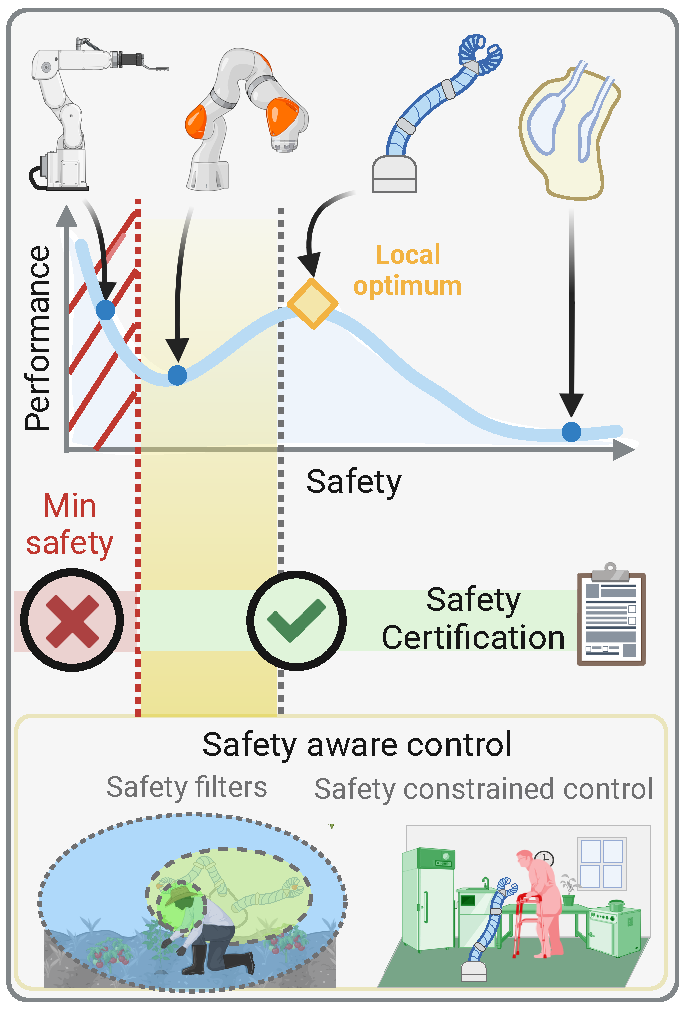
\includegraphics[width=0.65\linewidth]{safetymetric/figures/safety_metric_applications.pdf}
    \caption{Future applications that a quantitative safety metric for soft robots would enable. \textbf{Top:} Here, we showcase how the safety metric could be used for \emph{safety-aware design optimization} and, particularly, for analyzing and exploiting the performance vs. safety tradeoff. Subsequently, the safety metric could be used for certifying a given design as \emph{safe} for the respective application. \textbf{Bottom:} The safety metric could also be used for \emph{safety-aware control} - either by filtering the outputs of the controller without safety guarantees or by explicitly including the safety requirements as constraints during the optimization of the control input sequence (e.g., \gls{MPC}, \glspl{CBF}).}
    \label{fig:safetymetric:safety_metric_applications}
\end{figure}

\subsection{Potential Applications for a Safety Metric}\label{sub:safetymetric:safety_metric_applications}
% We envision a safety metric for soft robots to unlock a variety of applications that we showcase in Fig.~\ref{fig:safety_metric_applications}, and that can be grouped into the domains of \emph{safety-aware control} and \emph{safety-aware design}.
We envision a safety metric for soft robots that will enable a variety of applications, as illustrated in Fig.~\ref{fig:safetymetric:safety_metric_applications}. These applications can be categorized into two main domains: \emph{safety-aware control} and \emph{safety-aware design}.

% In the domain of \emph{safety-aware control}, we assume the soft robotic design to be given, and we strive to control the actions of the soft robot in such a way that the achieved safety level remains within an acceptable range. We remark that this does not exclude contact or even collision with the environment. Instead, we strive to guarantee that these collisions do not cause any (significant) injuries. Examples include \emph{safety filters}~\cite {bertino2023prescribed} that allow us to use performant control policies that do not explicitly consider the safety constraints (e.g., RL) and still guarantee safety by filtering/saturating the control input. Alternative techniques such as MPC~\citep{hewing2020learning} or Control Barrier Functions~\citep{ames2016control}, which we refer to as \emph{safety-constrained control}, allow us to take the safety constraints directly into account when devising the control input.
In the realm of \emph{safety-aware control}, we assume the soft robotic design is already established and focus on controlling its actions to maintain an acceptable safety level. This approach does not preclude contact or collisions with the environment; rather, it ensures that such interactions do not result in significant injuries. Examples include \emph{safety filters}~\citep{bertino2023prescribed}, which allow the use of high-performance control policies, such as \gls{RL}, that do not explicitly account for safety constraints while still guaranteeing safety by filtering or saturating the control input. Alternative methods like \gls{MPC}~\citep{hewing2020learning, pupa2024efficient} or \glspl{CBF}~\citep{ames2016control, ferraguti2020control}—referred to as \emph{safety-constrained control}—integrate safety constraints directly into the control strategy.

% Another avenue that would be unlocked by a safety metric is \emph{safety-aware design}, which would include assessing an integrated soft robot design for its safety. Specifically, we consider here two subcategories: \emph{safety-aware design optimization} would consider safety when developing/optimizing the soft robot design either by means of inequality constraints (i.e., a minimum safety needs to be guaranteed) or by maximizing safety through the cost function.
% After a design is finalized, \emph{safety certification} would allow manufacturers to certify their product as being sufficiently safe for the respective applications (e.g., healthcare, agri-food, manufacturing, etc.). This is well-aligned with established safety standards for collaborative rigid robots as defined in ISO/TS 15066:2016~\citep{iso2016collaborative}.
Another promising direction unlocked by a safety metric is \emph{safety-aware design}, which involves evaluating an integrated soft robot design for its safety. We see this as comprising two subcategories: \emph{safety-aware design optimization}, which incorporates safety into the design process either through inequality constraints (ensuring a minimum safety level) or by maximizing safety via the cost function; and \emph{safety certification}, where, after a design is finalized, manufacturers can certify that their product meets the necessary safety standards for specific applications (e.g., healthcare, agri-food, manufacturing, etc.). This approach aligns well with established safety standards for collaborative rigid robots as defined in ISO/TS 15066:2016~\citep{iso2016collaborative}.

\subsection{Requirements for a Soft Robotic Safety Metric}\label{sub:safetymetric:safety_metric_requirements}
% In the following, we will list some requirements that, in our opinion, a safety metric needs to meet in order to be well suited for the applications listed in Sec.~\ref{sub:safetymetric:safety_metric_applications}.
% First (1), the metric shall consider the dynamics inherent to continuum soft robots and their particular characteristics. For example, one of the main differences between rigid and soft manipulators is that free-moving joints with integrated motors are replaced by an elastic structure that deforms under the influence of internal actuation and external forces. Therefore, any safety metric needs to crucially consider the elastic and inertial characteristics of the soft robot that are generated by the distributed material along its backbone.
% Secondly (2), the safety metric shall consider not just collision at the end-effector but instead anywhere along the body of the soft robot. This is a significant difference to the existing safety metrics for rigid/collaborative robots, which, for simplicity, usually only consider collisions at the end-effector as we would expect there the largest motion velocities~\citep{haddadin2011safe, iso2016collaborative}. Instead, soft robots exhibit large Cartesian stiffnesses close to their proximal end, thus requiring us to consider the safety of collisions anywhere along the backbone.
% Next, (3) any simplifying assumptions shall lead to a conservative estimate of the achieved safety. For example, soft robot models underlying the safety metric would likely use a finite-dimensional approximation of the continuum shape; instead, in reality, flexible structures such as soft robots exhibit infinite degrees of freedom~\citep{della2023model, armanini2023soft}. Therefore, we would like any safety metric making use of finite-dimensional approximations to underestimate instead of overestimate the safety of the design.
% Fourthly (4), the computation of the safety metric shall be computationally tractable, which is essential for safety-aware control and design applications, where evaluations on the scale of sub-seconds and seconds are necessary.
% Finally, we end with a few desirable characteristics: (5) some applications, such as safety-aware control or safety-aware design, might benefit from the differentiability of the safety metric with respect to design parameters, robot states, and control inputs; (6) ideally, the safety metric shall also consider how \emph{safe} the soft robot's design (e.g., friendly-looking) and behavior (e.g., smooth and predictable movements) is perceived by the user. In addition to user studies, the evaluation of this metric might be assisted by VLMs.
In the following, we outline several requirements that, in our opinion, a safety metric must satisfy to be well-suited for the applications described in Sec.~\ref{sub:safetymetric:safety_metric_applications}. First (1), the metric should account for the dynamics inherent to continuum soft robots and their unique characteristics. For example, a primary difference between rigid and soft manipulators is that free-moving joints with integrated motors are replaced by a compliant structure that deforms under internal actuation and external forces. Consequently, any safety metric must consider the elastic and inertial properties generated by the distributed material along the robot’s backbone.
%
Secondly (2), the safety metric must evaluate collisions occurring anywhere along the soft robot’s body—not just at the end-effector. This represents a significant departure from existing safety metrics for rigid or collaborative robots, which often focus solely on the end-effector due to its typically higher motion velocities~\citep{haddadin2009requirements, haddadin2011safe, iso2016collaborative}. In contrast, soft robots exhibit high Cartesian stiffness near their proximal end, making it necessary to assess safety along the entire structure.
% 
Next (3), any simplifying assumptions should yield a conservative safety estimate. For instance, while soft robot models used in the metric might employ a finite-dimensional approximation of the continuum shape, in reality, these flexible structures possess infinite degrees of freedom~\citep{della2023model, armanini2023soft}. Therefore, a safety metric based on such approximations should tend to underestimate rather than overestimate the design’s safety.
% 
Fourthly (4), the computation of the safety metric must be tractable, which is essential for safety-aware control and design applications that require evaluations on sub-second to second timescales, respectively.
% 
Finally, we highlight a few desirable characteristics: (5) in applications such as safety-aware control or design, it is advantageous if the safety metric is differentiable with respect to design parameters, robot states, and control inputs; and (6) ideally, the metric should also reflect how “safe” the soft robot’s design (e.g., its friendly appearance) and behavior (e.g., smooth and predictable movements) are perceived by users. In addition to user studies, the evaluation of this metric might be enhanced by leveraging \glspl{VLM}~\citep{touvron2023llama, grattafiori2024llama}.